\documentclass{beamer}

\mode<presentation>
{
  \usetheme{default}
  \usecolortheme{default}
  \usefonttheme{default}
  \setbeamertemplate{navigation symbols}{}
  \setbeamertemplate{caption}[numbered]
  \setbeamertemplate{footline}[page number]
  \setbeamercolor{frametitle}{fg=white}
  \setbeamercolor{footline}{fg=black}
} 

\usepackage[english]{babel}
\usepackage[utf8x]{inputenc}
\usepackage{tikz}
\usepackage{listings}
\usepackage{courier}
\usepackage{array}
\usepackage{bold-extra}
\usepackage{minted}
\usepackage{transparent}

\xdefinecolor{darkblue}{rgb}{0.1,0.1,0.7}
\xdefinecolor{darkgreen}{rgb}{0,0.5,0}
\xdefinecolor{darkgrey}{rgb}{0.35,0.35,0.35}
\xdefinecolor{darkorange}{rgb}{0.8,0.5,0}
\xdefinecolor{darkred}{rgb}{0.7,0,0}
\xdefinecolor{dianablue}{rgb}{0.18,0.24,0.31}
\definecolor{commentgreen}{rgb}{0,0.6,0}
\definecolor{stringmauve}{rgb}{0.58,0,0.82}

\lstset{ %
  backgroundcolor=\color{white},      % choose the background color
  basicstyle=\ttfamily\small,         % size of fonts used for the code
  breaklines=true,                    % automatic line breaking only at whitespace
  captionpos=b,                       % sets the caption-position to bottom
  commentstyle=\color{commentgreen},  % comment style
  escapeinside={\%*}{*)},             % if you want to add LaTeX within your code
  keywordstyle=\color{blue},          % keyword style
  stringstyle=\color{stringmauve},    % string literal style
  showstringspaces=false,
  showlines=true
}

\lstdefinelanguage{scala}{
  morekeywords={abstract,case,catch,class,def,%
    do,else,extends,false,final,finally,%
    for,if,implicit,import,match,mixin,%
    new,null,object,override,package,%
    private,protected,requires,return,sealed,%
    super,this,throw,trait,true,try,%
    type,val,var,while,with,yield},
  otherkeywords={=>,<-,<\%,<:,>:,\#,@},
  sensitive=true,
  morecomment=[l]{//},
  morecomment=[n]{/*}{*/},
  morestring=[b]",
  morestring=[b]',
  morestring=[b]"""
}

\title[2017-05-11-dshep]{\bf \LARGE Data Plumbing}
\author{Jim Pivarski}
\institute{Princeton University -- DIANA}
\date{May 11, 2017}

\begin{document}

\logo{\pgfputat{\pgfxy(0.11, 8)}{\pgfbox[right,base]{\tikz{\filldraw[fill=dianablue, draw=none] (0 cm, 0 cm) rectangle (50 cm, 1 cm);}}}\pgfputat{\pgfxy(0.11, -0.6)}{\pgfbox[right,base]{\tikz{\filldraw[fill=dianablue, draw=none] (0 cm, 0 cm) rectangle (50 cm, 1 cm);}
\includegraphics[height=0.99 cm]{diana-hep-logo.png}\tikz{\filldraw[fill=dianablue, draw=none] (0 cm, 0 cm) rectangle (4.9 cm, 1 cm);}}}}

\usebackgroundtemplate{{\transparent{0.15}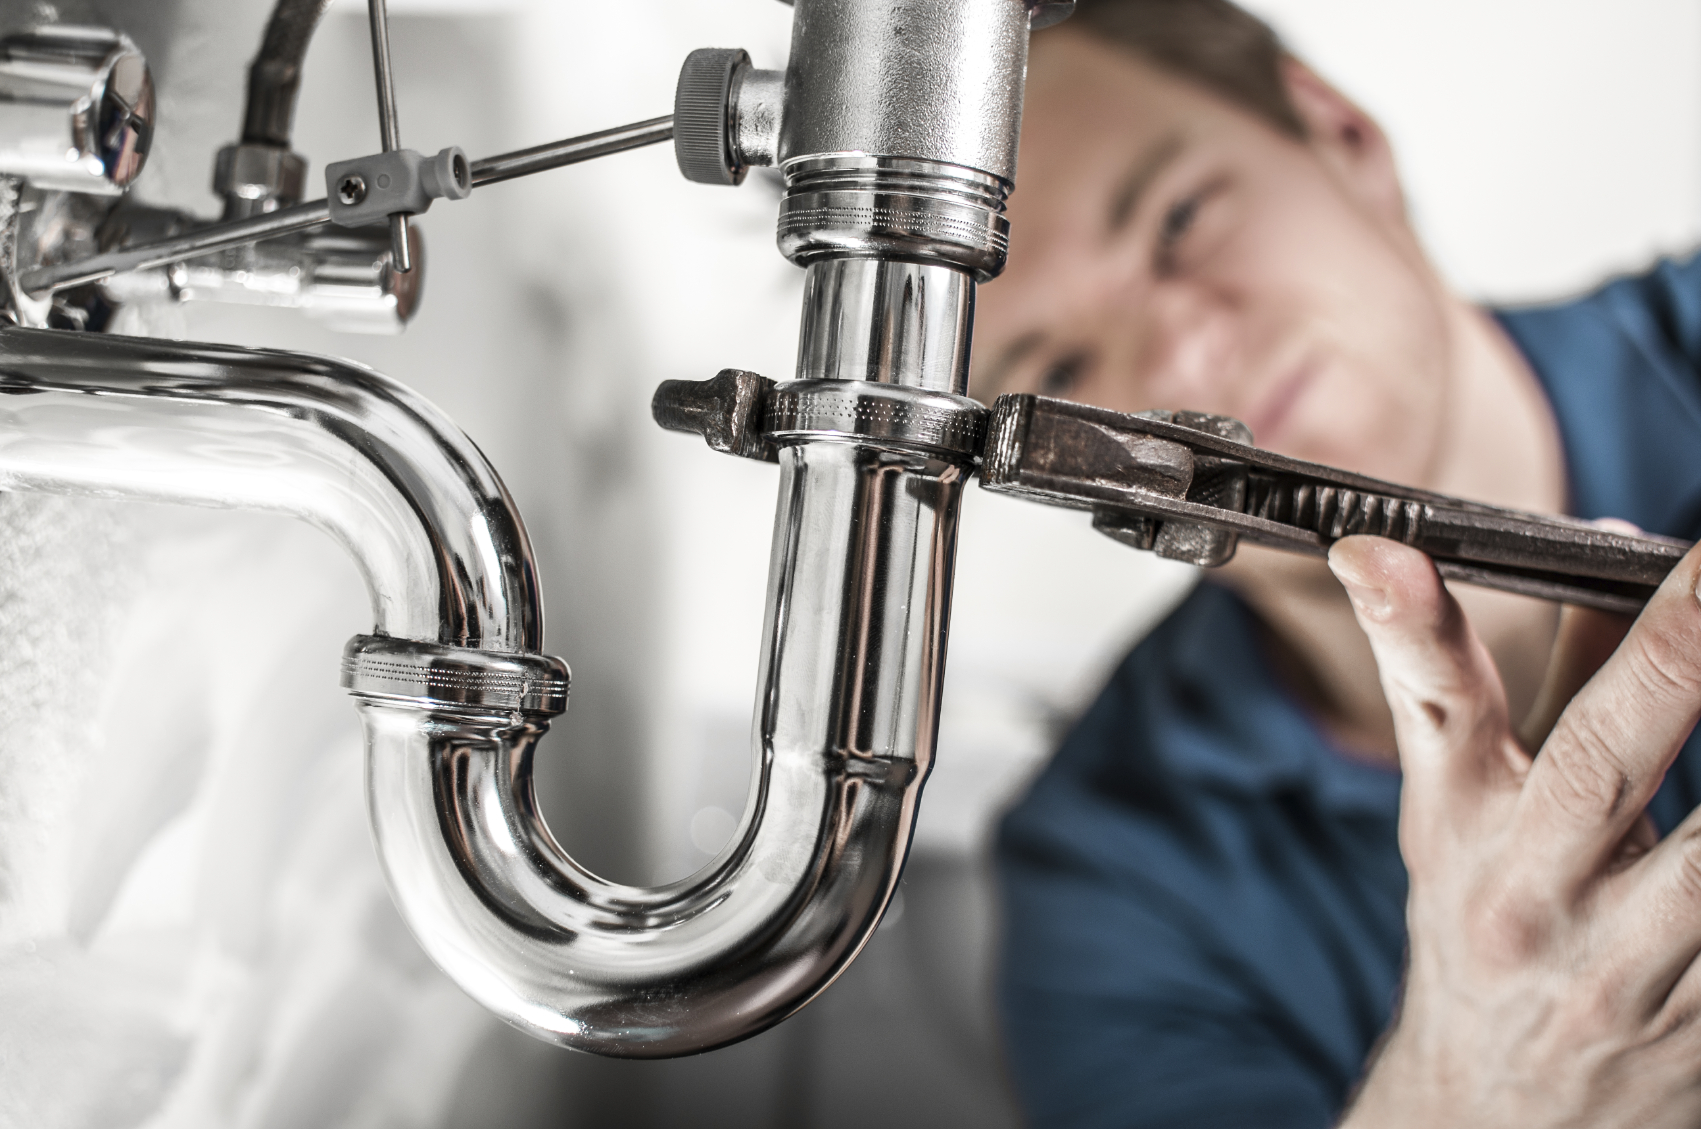
\includegraphics[width=\paperwidth,height=\paperheight]{plumbing.jpg}}}

\begin{frame}
  \titlepage
\end{frame}

\usebackgroundtemplate{}

\logo{\pgfputat{\pgfxy(0.11, 8)}{\pgfbox[right,base]{\tikz{\filldraw[fill=dianablue, draw=none] (0 cm, 0 cm) rectangle (50 cm, 1 cm);}
\includegraphics[height=1 cm]{diana-hep-logo.png}}}}

% Uncomment these lines for an automatically generated outline.
%\begin{frame}{Outline}
%  \tableofcontents
%\end{frame}

%%%%%%%%%%%%%%%%%%%%%%%%%%%%%%%%%%%%%%%%%%%%%%%%%%%%%%%

\begin{frame}{Why bother?}
We're all here because we think that HEP can benefit from machine learning techniques.

\vfill
\uncover<2->{The most advanced techniques are being developed outside of HEP using (what are becoming) industry standard tools.}

\vfill
\uncover<3->{\textcolor{darkblue}{Problem:} our HEP protocols and formats won't work with them without some modification or export.}

\vfill
\uncover<4->{\textcolor{darkblue}{This talk is about moving data from one format to another.}}
\end{frame}

\begin{frame}{}

\only<1>{\mbox{\hspace{-1 cm}
\includegraphics[width=1.2\linewidth]{diana-hep.png}}}
\only<2>{\mbox{\hspace{-1 cm}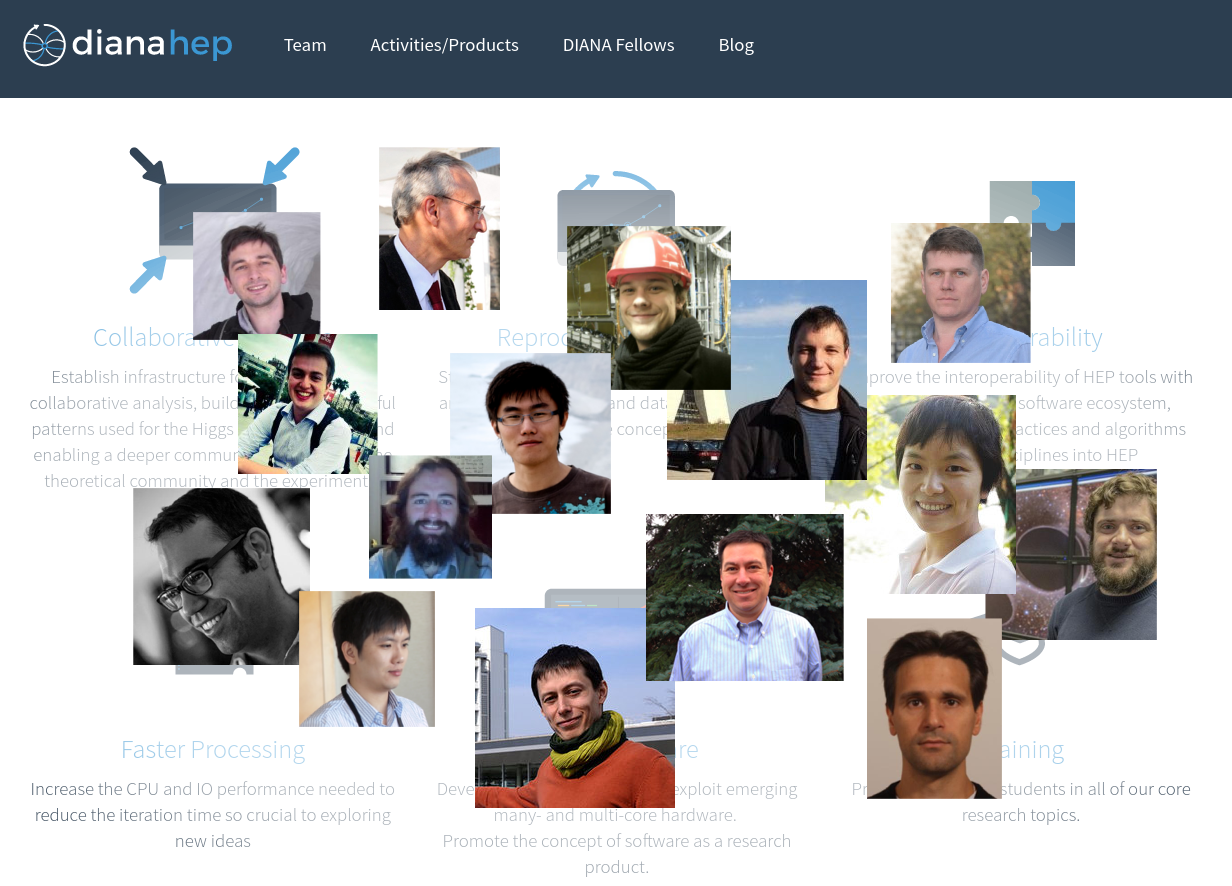
\includegraphics[width=1.2\linewidth]{diana-hep2.png}}}

\end{frame}

\begin{frame}{Goals of this talk}
\Large
\begin{itemize}\setlength{\itemsep}{0.5 cm}
\item \textcolor{darkblue}{make \underline{you} aware of what's possible}
\item \textcolor{darkblue}{introduce some software tools}
\item \textcolor{darkblue}{invite you to tell \underline{me} what's needed.}
\end{itemize}
\end{frame}

%% \begin{frame}{}
%% \begin{center}
%% \LARGE \textcolor{darkblue}{ROOT and Numpy}
%% \end{center}
%% \end{frame}

%% \begin{frame}[frame]{root\_numpy}
%% \vfill
%% \begin{columns}[t]
%% \column{0.5\linewidth}
%% ROOT is the standard for HEP data storage and processing.
%% \column{0.5\linewidth}
%% Numpy is the standard for the scientific Python ecosystem, including TensorFlow, Keras, {\small PyTorch,} {\footnotesize DyNet,} {\scriptsize MinPy,} {\tiny MXNet\ldots}
%% \end{columns}

%% \vfill
%% \begin{uncoverenv}<2->
%% 
\includegraphics[height=2.5 cm]{scikit-hep_logo_800.png}

%% \vspace{-2.5 cm}
%% \hfill \begin{minipage}{0.7\linewidth}
%% root\_numpy from Scikit-HEP provides high-level translation from ROOT TTrees to Numpy arrays and back.

%% \vspace{0.5 cm}
%% \textcolor{blue}{\underline{\url{http://scikit-hep.org/root_numpy/}}}
%% \end{minipage}
%% \end{uncoverenv}
%% \end{frame}

%% \begin{frame}[fragile]{Examples}
%% \small
%% \begin{minted}{python}
%% import root_numpy

%% # get an array from a ROOT file named by string
%% filename = root_numpy.testdata.get_filepath("test.root")
%% array1 = root_numpy.root2array(filename, "tree")

%% # or get an array from a PyROOT TFile/TTree
%% import ROOT
%% rootfile = ROOT.TFile(filename)
%% roottree = rootfile.Get("tree")
%% array2 = root_numpy.tree2array(roottree)
%% \end{minted}

%% \vspace{0.5 cm}
%% \begin{uncoverenv}<2->
%% {\normalsize Use {\tt TTree::Draw} syntax to transform branches and cut events.}

%% \begin{minted}{python}
%% array3 = root_numpy.tree2array(roottree,
%%     branches=["x", "y", "sqrt(y)", "TMath::Landau(x)"],
%%     selection="z > 0")
%% \end{minted}
%% \end{uncoverenv}
%% \end{frame}

%% \begin{frame}{Worth noting\ldots}
%% \vspace{0.25 cm}
%% \begin{itemize}\setlength{\itemsep}{0.5 cm}
%% \item Although root\_numpy loads whole branches into memory as arrays, it would be possible to extend it to streaming C++ APIs (hint: TensorFlow).

%% \item There are other extensions ``out there,'' such as this one:
%% \begin{center}
%% \textcolor{blue}{\underline{\url{https://github.com/ibab/root_pandas}}}
%% \end{center}

%% \item Scikit-HEP is a metapackage (developers below) to try to make things like this easier to find.

%% \footnotesize
%% \vspace{0.25 cm}
%% Noel Dawe (University of Melbourne), Vanya Belyaev (ITEP), Sasha Mazurov (University of Birmingham), Eduardo Rodrigues (University of Cincinnati), David Lange (Princeton University), and myself.
%% \end{itemize}
%% \end{frame}

%% \begin{frame}{}
%% \begin{center}
%% \LARGE \textcolor{darkblue}{direct to Numpy}
%% \end{center}
%% \end{frame}

%% \begin{frame}{Skip the middleman}
%% \vspace{0.25 cm}
%% root\_numpy is great if you have a lot of ROOT files and need to analyze them in Python.

%% \vspace{0.25 cm}
%% \uncover<2->{But if you don't already have the ROOT files, generating and then converting them is awkward, especially if the dataset is large.}

%% \begin{uncoverenv}<3->
%% \vspace{0.25 cm}
%% \begin{block}{The Numpy format is extremely simple.}
%% \begin{itemize}\setlength{\itemsep}{0.25 cm}
%% \item<4-> a Numpy array is a plain C array interpreted by metadata {\small (data type,} {\footnotesize number of elements,} {\scriptsize endianness,} {\tiny C vs.\ Fortran-style stride\ldots)}
%% \begin{itemize}
%% \item you can wrap any region of memory as a Numpy array
%% \end{itemize}

%% \item<5-> a Numpy file is a literal copy of the array with a header
%% \begin{itemize}
%% \item you can write Numpy files with minimal code
%% \end{itemize}

%% \end{itemize}
%% \end{block}
%% \end{uncoverenv}
%% \end{frame}

%% \begin{frame}[fragile]{Examples of wrapping arrays}
%% \vspace{0.25 cm}
%% If PyROOT gives you an {\tt array.array}, wrap it like this:

%% \small
%% \begin{minted}{python}
%%     import numpy
%%     numpy_array = numpy.frombuffer(array_from_root)
%% \end{minted}

%% \normalsize
%% Now it has Numpy powers.

%% \begin{uncoverenv}<2->
%% \vspace{0.25 cm}
%% As long as you perform in-place operations, like

%% \small
%% \begin{minted}{python}
%%     # overwrite all elements x with sin(x)
%%     numpy.sin(numpy_array, numpy_array)
%%     # set all values to 3.14
%%     numpy_array[:] = 3.14
%% \end{minted}

%% \normalsize
%% it will modify the same memory that ROOT is looking at.
%% \end{uncoverenv}

%% \begin{uncoverenv}<3->
%% \vspace{0.25 cm}
%% \textcolor{darkblue}{With great power comes great responsibility:} if ROOT deletes this array and you continue to modify it, you will corrupt memory, causing a segmentation fault {\it at best.}
%% \end{uncoverenv}
%% \end{frame}

%% \begin{frame}[fragile]{Examples of wrapping arrays}
%% You can split a Python script into parallel processes using its builtin {\tt multiprocessing} module. These processes can share a block of memory, which you can wrap with Numpy.

%% \vspace{0.25 cm}
%% See \textcolor{blue}{\underline{\url{https://goo.gl/NPwcSL}}} for an example.
%% \end{frame}

%% \begin{frame}[fragile]{Examples of wrapping arrays}
%% \vspace{0.5 cm}
%% \hfill 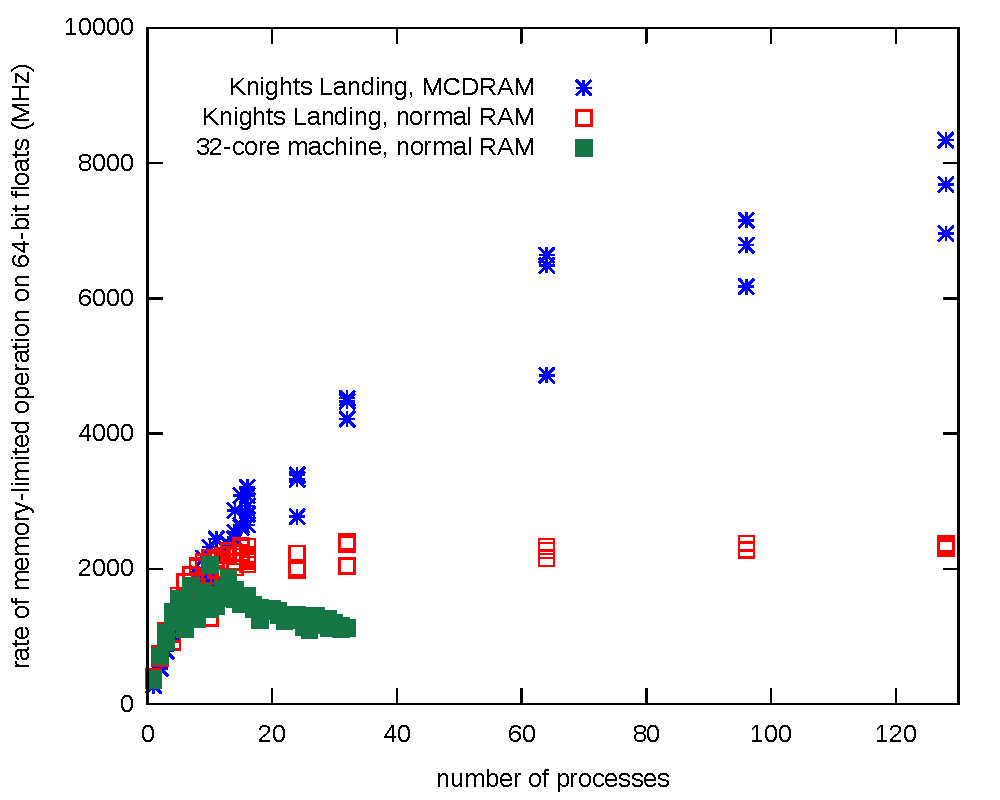
\includegraphics[height=3.5 cm]{knl-scaling.pdf}

%% \vspace{-3.5 cm}
%% Even use non-standard allocators \\ (this one allocates memory on \\ Knight's Landing MCDRAM).

%% \vspace{0.25 cm}
%% \scriptsize
%% \begin{minted}{python}
%% import ctypes
%% import numpy

%% ZILLION = 1000000

%% libnuma = ctypes.cdll.LoadLibrary("libnuma.so")
%% libnuma.numa_alloc_local.restype = ctypes.POINTER(ctypes.c_double)
%% ptr = libnuma.numa_alloc_local(ctypes.c_size_t(ZILLION))

%% ptr.__array_interface__ =
%%     {"version": 3,
%%      "typestr": numpy.ctypeslib._dtype(type(ptr.contents)).str,
%%      "data": (ctypes.addressof(ptr.contents), False),
%%      "shape": (ZILLION,)}

%% asarray = numpy.array(ptr, copy=False)
%% \end{minted}
%% \end{frame}

%% \begin{frame}[fragile]{Quick 'n easy way to write to Numpy files}
%% \begin{center}
%% \textcolor{blue}{\underline{\url{https://github.com/diana-hep/c2numpy}}}
%% \end{center}

%% Pure-header C library: drop it in and write Numpy files.

%% \vspace{0.25 cm}
%% \scriptsize
%% \begin{minted}{c++}
%% #include "c2numpy.h"

%% c2numpy_init(&writer, "output/tracks", 1000);
%% c2numpy_addcolumn(&writer, "pt", C2NUMPY_FLOAT64);
%% c2numpy_addcolumn(&writer, "eta", C2NUMPY_FLOAT64);
%% c2numpy_addcolumn(&writer, "phi", C2NUMPY_FLOAT64);
%% c2numpy_addcolumn(&writer, "dxy", C2NUMPY_FLOAT64);
%% c2numpy_addcolumn(&writer, "dz", C2NUMPY_FLOAT64);

%% ...

%% for (auto track = tracks->cbegin();
%%      track != tracks->end();
%%      ++track) {
%%   c2numpy_float64(&writer, track->pt());
%%   c2numpy_float64(&writer, track->eta());
%%   c2numpy_float64(&writer, track->phi());
%%   c2numpy_float64(&writer, track->dxy());
%%   c2numpy_float64(&writer, track->dz());
%% }
%% \end{minted}
%% \end{frame}

\begin{frame}{}
\begin{center}
\LARGE \textcolor{darkblue}{industry standard formats}

\vspace{0.25 cm}
\textcolor{darkblue}{\Large Avro/ProtoBuf/Thrift, Parquet, Arrow/Feather}
\end{center}
\end{frame}

\begin{frame}{What about nested structure?}
Numpy isn't appropriate (efficient) for anything but flat-flat ntuples: strictly columns of numbers, no {\tt\small std::vector<double>}!






\end{frame}



\begin{frame}{}
\begin{center}
\LARGE \textcolor{darkblue}{Spark and the JVM}
\end{center}
\end{frame}

\begin{frame}{}
\begin{center}
\LARGE \textcolor{darkblue}{moving fitted models}
\end{center}
\end{frame}

\begin{frame}{Conclusing remarks}

\end{frame}

\end{document}
